% Figure: Heliomorphic Function Structure
% Visualizes the radial-phase coupling and gravitational field interactions

\begin{figure}[ht]
\centering
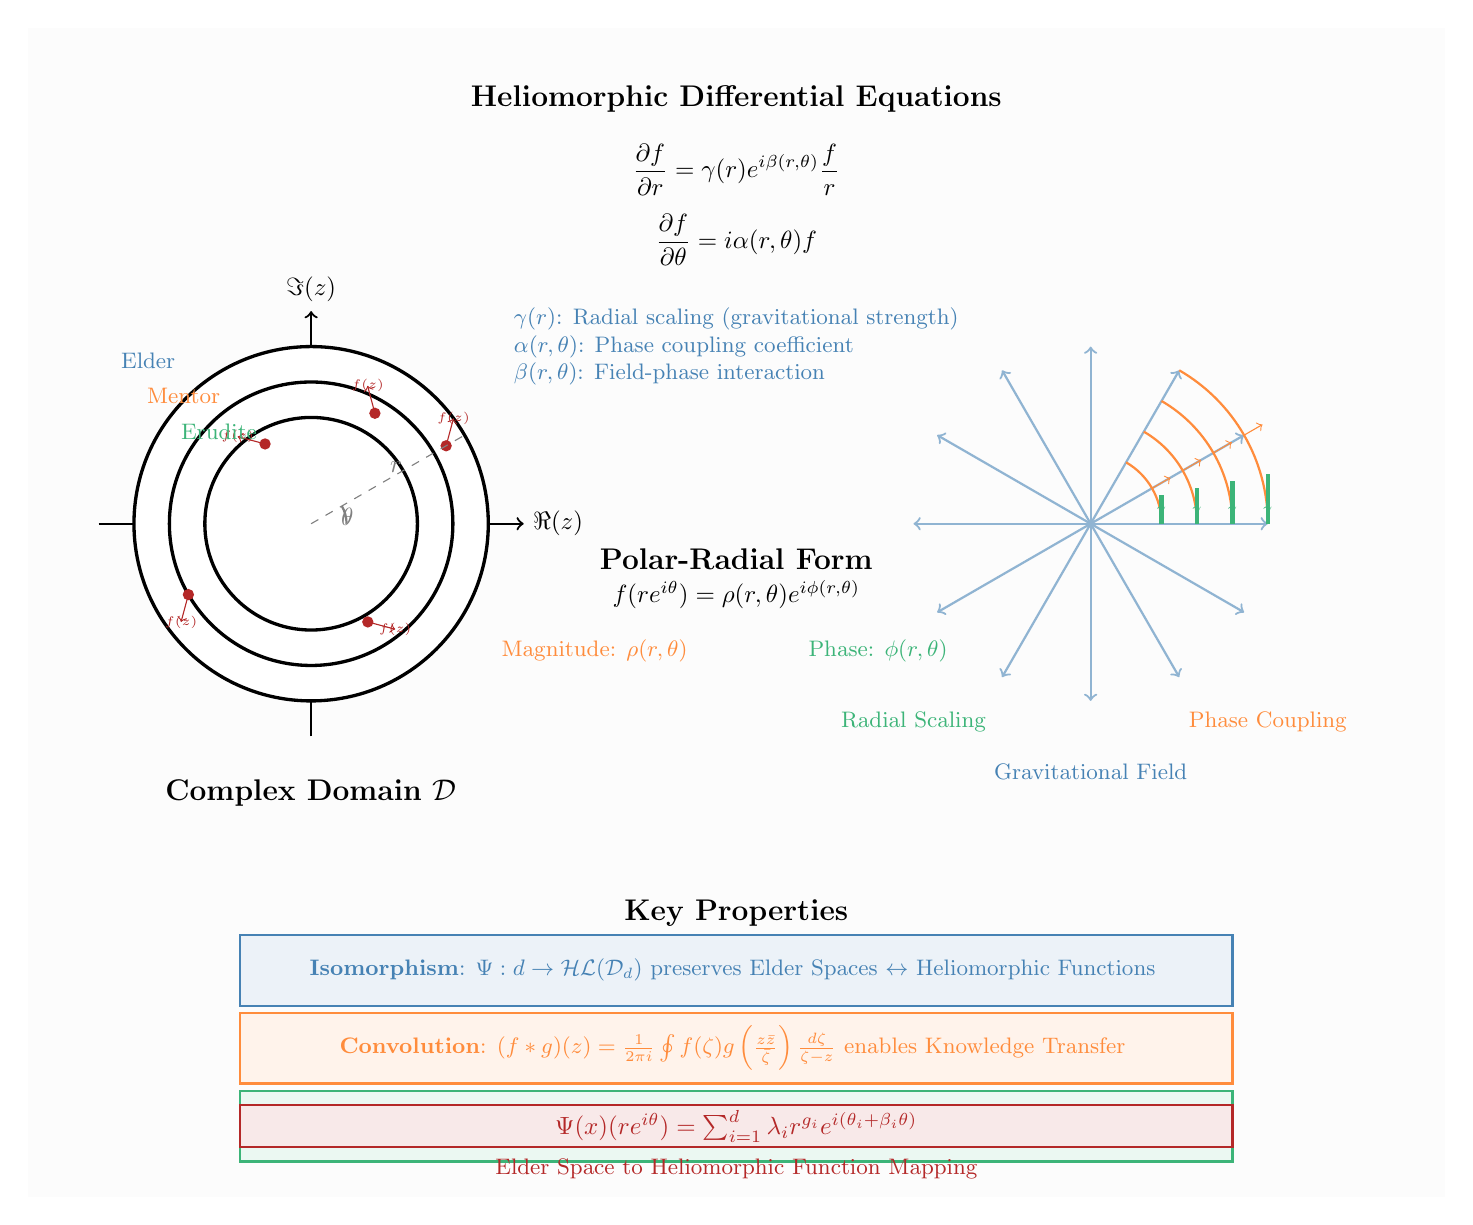
\begin{tikzpicture}[scale=0.9, every node/.style={transform shape}]

% Define colors matching Elder theme
\definecolor{ElderBlue}{RGB}{70, 130, 180}
\definecolor{MentorOrange}{RGB}{255, 140, 60}
\definecolor{EruditeGreen}{RGB}{60, 180, 120}
\definecolor{LightGray}{RGB}{240, 240, 240}
\definecolor{DeepRed}{RGB}{180, 40, 40}

% Background
\fill[LightGray!20] (-10, -9.5) rectangle (10, 7);

% Left side: Complex domain visualization
\begin{scope}[shift={(-6, 0)}]
    % Complex plane axes
    \draw[black, thick, ->] (-3, 0) -- (3, 0) node[right] {$\Re(z)$};
    \draw[black, thick, ->] (0, -3) -- (0, 3) node[above] {$\Im(z)$};
    
    % Annular regions representing gravitational strata
    \foreach \r/\color/\alpha in {2.5/ElderBlue/0.15, 2/MentorOrange/0.15, 1.5/EruditeGreen/0.15} {
        \draw[\color, very thick, fill=\color!\alpha] (0,0) circle (\r);
    }
    
    % Sample points and their heliomorphic values
    \foreach \angle/\r in {30/2.2, 60/1.8, 120/1.3, 210/2.0, 300/1.6} {
        \coordinate (P) at (\angle:\r);
        \fill[DeepRed] (P) circle (0.08);
        \draw[DeepRed, ->] (P) -- +(\angle+45:0.4) node[font=\tiny] {$f(z)$};
    }
    
    % Radial and angular coordinates
    \draw[dashed, gray] (0,0) -- (30:2.5);
    \draw[gray, thick] (0.5,0) arc (0:30:0.5);
    \node[gray, right] at (0.3,0.1) {$\theta$};
    \node[gray, above] at (1.2,0.6) {$r$};
    
    % Domain label
    \node[black, font=\large\bfseries] at (0, -3.8) {Complex Domain $\mathcal{D}$};
    \node[ElderBlue, font=\small] at (-2.3, 2.3) {Elder};
    \node[MentorOrange, font=\small] at (-1.8, 1.8) {Mentor};
    \node[EruditeGreen, font=\small] at (-1.3, 1.3) {Erudite};
\end{scope}

% Center: Heliomorphic differential equations
\begin{scope}[shift={(0, 3)}]
    \node[black, font=\large\bfseries] at (0, 3) {Heliomorphic Differential Equations};
    
    % First equation
    \node[black, font=\normalsize] at (0, 2) {$\displaystyle\frac{\partial f}{\partial r} = \gamma(r)e^{i\beta(r,\theta)}\frac{f}{r}$};
    
    % Second equation  
    \node[black, font=\normalsize] at (0, 1) {$\displaystyle\frac{\partial f}{\partial \theta} = i\alpha(r,\theta)f$};
    
    % Parameter descriptions
    \node[ElderBlue, font=\small, align=left] at (0, -0.5) {
        $\gamma(r)$: Radial scaling (gravitational strength)\\
        $\alpha(r,\theta)$: Phase coupling coefficient\\
        $\beta(r,\theta)$: Field-phase interaction
    };
\end{scope}

% Center: Polar-radial form
\begin{scope}[shift={(0, -1)}]
    \node[black, font=\large\bfseries] at (0, 0.5) {Polar-Radial Form};
    \node[black, font=\normalsize] at (0, 0) {$f(re^{i\theta}) = \rho(r,\theta)e^{i\phi(r,\theta)}$};
    
    % Component descriptions
    \node[MentorOrange, font=\small] at (-2, -0.8) {Magnitude: $\rho(r,\theta)$};
    \node[EruditeGreen, font=\small] at (2, -0.8) {Phase: $\phi(r,\theta)$};
\end{scope}

% Right side: Gravitational coupling visualization
\begin{scope}[shift={(5, 0)}]
    % Gravitational field lines
    \foreach \angle in {0, 30, 60, 90, 120, 150, 180, 210, 240, 270, 300, 330} {
        \draw[ElderBlue!60, thick, ->] (0,0) -- (\angle:2.5);
    }
    
    % Phase coupling arrows
    \foreach \r in {1, 1.5, 2, 2.5} {
        \draw[MentorOrange, thick] (\r,0) arc (0:60:\r);
        \draw[MentorOrange, ->] (30:\r) -- +(30:0.3);
    }
    
    % Coupling strength indicators
    \foreach \r/\strength in {1/0.8, 1.5/1.0, 2/1.2, 2.5/1.4} {
        \draw[EruditeGreen, ultra thick] (0:\r) -- +(90:\strength*0.5);
        \node[EruditeGreen, font=\tiny] at (0:\r) [above] {$\gamma$};
    }
    
    % Labels
    \node[ElderBlue, font=\small] at (0, -3.5) {Gravitational Field};
    \node[MentorOrange, font=\small] at (2.5, -2.8) {Phase Coupling};
    \node[EruditeGreen, font=\small] at (-2.5, -2.8) {Radial Scaling};
\end{scope}

% Bottom: Heliomorphic properties
\begin{scope}[shift={(0, -8)}]
    \node[black, font=\large\bfseries] at (0, 2.5) {Key Properties};
    
    % Property boxes - stacked vertically with expanded width
    \draw[ElderBlue, thick, fill=ElderBlue!10] (-7, 1.2) rectangle (7, 2.2);
    \node[ElderBlue, font=\small, align=center] at (0, 1.7) {
        \textbf{Isomorphism}: $\Psi: \elder{d} \rightarrow \mathcal{HL}(\mathcal{D}_d)$ preserves Elder Spaces $\leftrightarrow$ Heliomorphic Functions
    };
    
    \draw[MentorOrange, thick, fill=MentorOrange!10] (-7, 0.1) rectangle (7, 1.1);
    \node[MentorOrange, font=\small, align=center] at (0, 0.6) {
        \textbf{Convolution}: $(f * g)(z) = \frac{1}{2\pi i} \oint f(\zeta) g\left(\frac{z\bar{z}}{\bar{\zeta}}\right) \frac{d\zeta}{\zeta - z}$ enables Knowledge Transfer
    };
    
    \draw[EruditeGreen, thick, fill=EruditeGreen!10] (-7, -1.0) rectangle (7, 0.0);
    \node[EruditeGreen, font=\small, align=center] at (0, -0.5) {
        \textbf{Hierarchical Domains}: $\mathcal{D}_{\text{Elder}} \subset \mathcal{D}_{\text{Mentor}} \subset \mathcal{D}_{\text{Erudite}}$ preserve abstraction levels
    };
\end{scope}

% Mathematical representation box
\begin{scope}[shift={(0, -8.5)}]
    \draw[DeepRed, thick, fill=DeepRed!10] (-7, -0.3) rectangle (7, 0.3);
    \node[DeepRed, font=\normalsize] at (0, 0) {
        $\Psi(x)(re^{i\theta}) = \sum_{i=1}^{d} \lambda_i r^{g_i} e^{i(\theta_i + \beta_i \theta)}$
    };
    \node[DeepRed, font=\small] at (0, -0.6) {Elder Space to Heliomorphic Function Mapping};
\end{scope}

\end{tikzpicture}

\caption{Heliomorphic Function Structure. The figure illustrates the key components of heliomorphic functions: (left) complex domain $\mathcal{D}$ with hierarchical annular regions corresponding to Elder, Mentor, and Erudite subspaces; (center) the defining differential equations and polar-radial form; (right) gravitational field-phase coupling visualization showing radial scaling $\gamma(r)$, phase coupling $\alpha(r,\theta)$, and field interaction $\beta(r,\theta)$. The bottom panel shows the fundamental isomorphism between Elder spaces and heliomorphic functions, enabling the bridge from abstract algebraic structures (Unit I) to functional realizations (Unit II).}
\label{fig:heliomorphic_structure}
\end{figure}